\documentclass{article}

\usepackage{epsfig}

\oddsidemargin= 0in
\evensidemargin= 0in
\topmargin=0in
\headheight= 0in
\headsep=0in
\parskip=6pt
\parindent=0pt
\setlength{\textheight}{9in}
\setlength{\textwidth}{6.5in}
\pagestyle{empty}

\newcommand{\classtitle}[2]{\noindent
{\large \bf 
\begin{tabbing} 
ECE198KL: Introduction to Computer Engineering II \` Spring 2013 \\
{#1} \` {#2}
\end{tabbing}
}
}
\newcommand{\classsect}[1]{{\large \bf {#1}}}
\newcommand{\classsubsect}[1]{\noindent{\bf {#1}:}}
\newcommand{\assntitle}[1]{\centerline{\large \bf {#1}}}
\newcommand{\url}[1]{\\ \centerline{\tt {#1}} \\}
\newcommand{\cmd}[1]{\centerline{\tt {#1}}}
\newcommand{\probnum}[2]{{\bf {#1}.  {#2}}}
\newcommand{\subprob}[1]{{\bf {#1}.}}
\newcommand{\reg}[1]{{\fix \%{#1}}}
\newcommand{\lowsig}[1]{$\overline{\mbox{{#1}}}$}

\newcommand{\ie}{{\em i.e.}}
\newcommand{\eg}{{\em e.g.}}
\newcommand{\etc}{{\em etc.}}

\newcommand{\mpline}{\vspace{6pt}}
\newcommand{\mpdone}{\vspace{-14pt}}
\newcommand{\st}{}

\setcounter{topnumber}{4}
\setcounter{bottomnumber}{4}
\renewcommand{\topfraction}{.9}
\renewcommand{\bottomfraction}{.9}
\setcounter{totalnumber}{6}
\renewcommand{\floatpagefraction}{.9}
\renewcommand{\dblfloatpagefraction}{.9}
\renewcommand{\dbltopfraction}{.9}
\setcounter{dbltopnumber}{4}
\renewcommand{\textfraction}{.1}

\newcommand{\twovert}[2]{\mbox{\arraycolsep 0pt \tabcolsep 0pt \begin{tabular}{c}{#1}\\{#2}\end{tabular}}}
\newcommand{\threevert}[3]{\mbox{\arraycolsep 0pt \tabcolsep 0pt \begin{tabular}{c}{#1}\\{#2}\\{#3}\end{tabular}}}
\newcommand{\fourvert}[4]{\mbox{\arraycolsep 0pt \tabcolsep 0pt \begin{tabular}{c}{#1}\\{#2}\\{#3}\\{#4}\end{tabular}}}
\newcommand{\fivevert}[5]{\mbox{\arraycolsep 0pt \tabcolsep 0pt \begin{tabular}{c}{#1}\\{#2}\\{#3}\\{#4}\\{#5}\end{tabular}}}



\begin{document}

\classtitle{Program 5}{due: 10 p.m. on Monday 18 February}
\bigskip
\assntitle{Codebreaker}
\bigskip

Your task this week is to implement the logic for a code-breaking game.
A code sequence of four numbers from~1 to~8 (colors in the graphical version)
is first chosen at random.
The player guesses a sequence of four numbers and is given feedback on each 
guess, including the number of values that appear in the same place
in the solution code (these we call {\em perfect matches}), and the
number of values that appear in a different place in the solution
code (these we call {\em misplaced matches}).
If the player manages to guess the correct sequence in twelve or fewer
guesses, they win the game.  Otherwise, they lose.

The objective for this week is for you to gain some experience with 
basic I/O, to implement code using multiple subroutines,
and to solve a problem that requires moderately
sophisticated reasoning and control logic.
%
The task here is thus somewhat more difficult than last week's.  
If you want to read ahead and
use arrays, feel free to do so.  One of the challenges requires use of 
arrays.  But the code should be fairly manageable without using arrays
(we wrote the solution that way, just to check).


\begin{minipage}{3.35in}
As always, routine details such as how to obtain the code and how to
hand in your program can be found in the specification for 
Program~1.  Instructions on targeting and making the Linux and Android
versions can be found in the specification for Program~4.\\ \mpline


\classsect{The Pieces}\mpline

We are using the same package to allow cross-compilation on different
platforms as well as support for the graphical user interface.  With
a number of image files and more sample tests, this week's distribution
is almost 150 files.  Again, however,  you again need only
look at three of those files---the rest serve to incorporate your
code into the graphical game and to allow you to build the game
as a text version on the lab machines or as a graphical version
on Android, Linux, Windows, or WebOS.\mpline

The three files that you should examine are a header file, the source
file that you must complete, and a standalone file that
creates a text version of the game and may help you debug your code 
before you build it into the graphical version.\mpline
\end{minipage}\hspace{.25in}%
\begin{minipage}{2.9in}
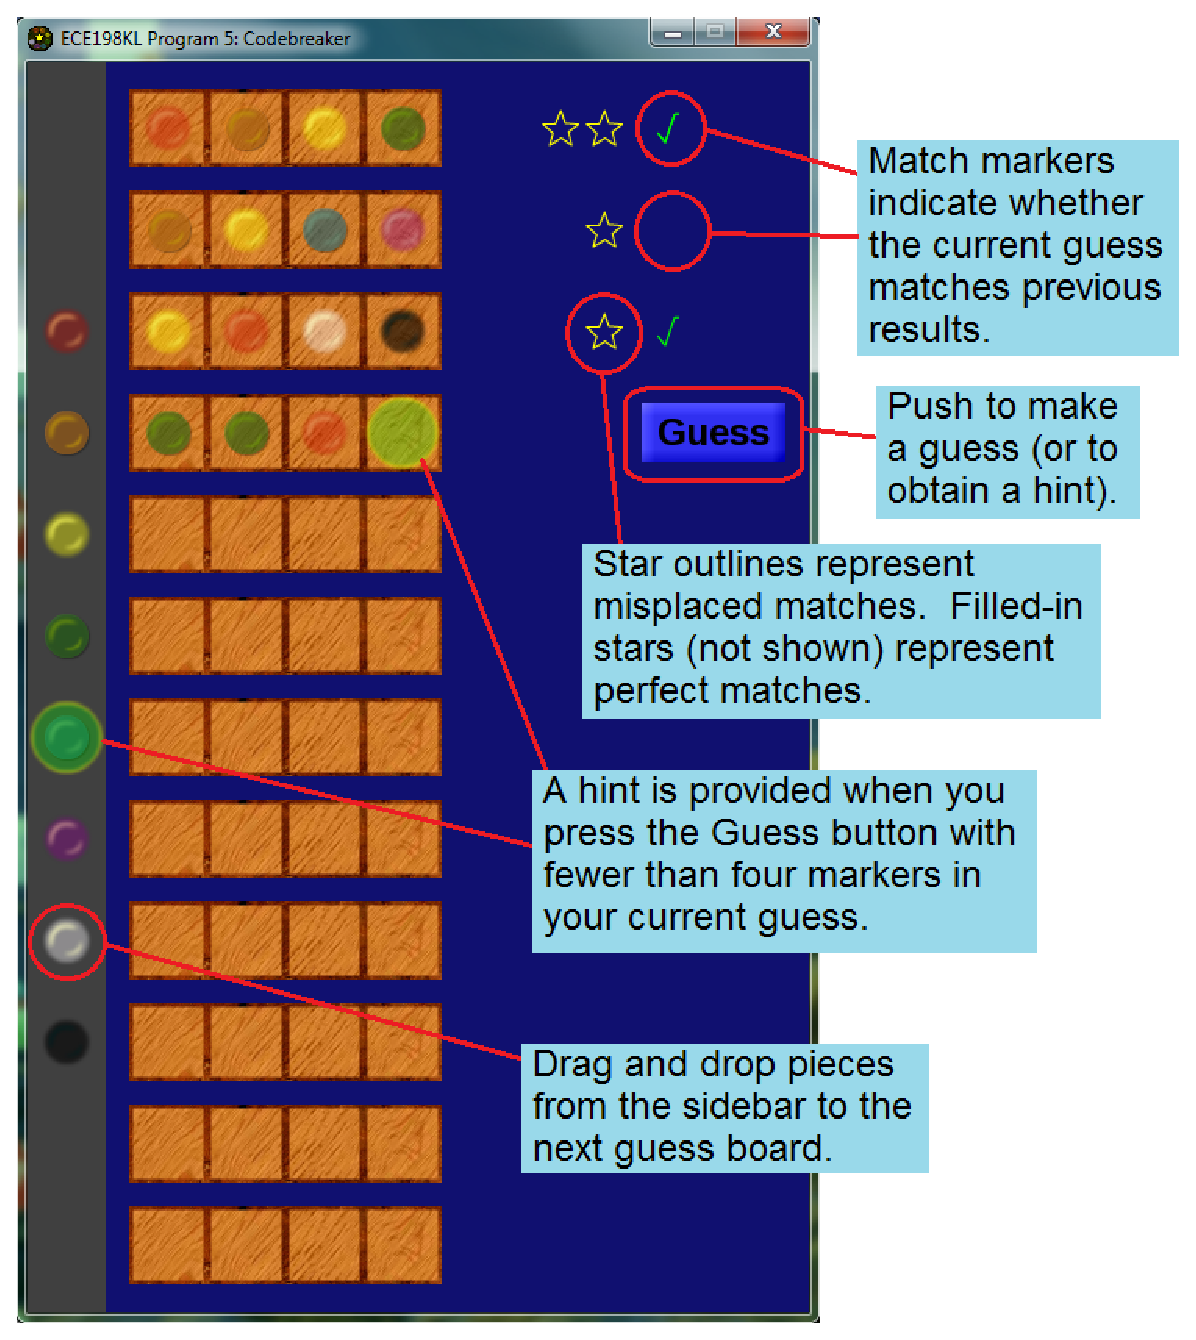
\epsfig{file=codebreaker.eps,width=2.9in}
\end{minipage}

Let's discuss each of these in a little more detail:

\begin{list}{x}{\setlength{\leftmargin}{1.5in}\setlength{\rightmargin}{0.5in}\setlength{\labelwidth}{1.25in}\setlength{\itemsep}{0pt}\setlength{\parskip}{0pt}\setlength{\parsep}{0pt}}
\item[{\tt jni/prog5.h}~~]{This header file provides function declarations
and descriptions of the functions that you must write for this assignment,
along with a description of the {\tt prog5\_printf} function that you must
use for printing output from your functions.}
\item[{\tt jni/prog5.c}~~]{The main source file for your code.
Function headers for all regular and challenge functions are provided
to help you get started.  We will work together on the {\tt set\_seed}
function in programming studio.  The next two, {\tt start\_game} 
and {\tt make\_guess}, are left for you to finish independently.
The last two, {\tt compare\_guesses} and {\tt get\_hint},
correspond to challenges.}
\item[{\tt text\_version.c}~~]{This file uses {\tt \#include} to
pull in the source file that you
must edit, but not the rest of the game package, then executes
your code as a text-mode game.
You may find this version easier to debug, and we have provided 
some test files as well as a gold (correct, fully operational) version
if you want to create more test outputs.  The text version does not
implement the challenges.}
\end{list}

We have also included some additional files for testing, but we leave 
discussion of those files
for the Testing section of this document.

In programming studio, we will discuss pseudo-random number generation
and the idea of error-checking user input, then develop the {\tt set\_seed}
function together to robustly translate user input into a well-defined
seed for the pseudo-random number generator.  

{\bf The rest of the assignment must be completed on your own.}
%
If you want to get started before Thursday, you can leave the implementation
of {\tt set\_seed} provided in the distribution and work on {\tt start\_game}
and {\tt make\_guess.}  Together with {\tt set\_seed}, these three functions
comprise the whole assignment for this week.\\

\classsect{Details}

You should read the descriptions of the functions in the header
file and peruse the function headers in the source file before you begin
coding.
%
For the {\tt set\_seed} routine that we will develop in programming studio,
the function signature appears below:

\protect{\mbox{\hspace{.25in}}}%
{\tt int32\_t set\_seed (const char* seed\_str);}

The function receives a string (a pointer to a character) as its input
and produces a \mbox{32-bit} signed integer as output.  The ``{\tt const}''
qualifier means that the routine is not allowed to change the contents 
of the string.  

We use the following two library calls to produce sequences of pseudo-random numbers:

\protect{\mbox{\hspace{.25in}}}%
{\tt void srand (unsigned int seed);}\\
\protect{\mbox{\hspace{.25in}}}%
{\tt int rand ();}

\begin{minipage}{4.8in}
In the graphical version of our game,
the value typed into the entry box shown to the right is delivered to
the {\tt set\_seed} function as a string when the player presses $<$Enter$>$.
The {\tt set\_seed} routine
must then check whether the string represents a number, and, if so,
use it to seed the pseudo-random number generator via a call 
to {\tt srand}.  Calls to {\tt rand} then produce pseudo-random numbers
in the range~$[0,2^{31}-1]$.
\end{minipage}\hspace{.25in}%
\begin{minipage}{1.45in}
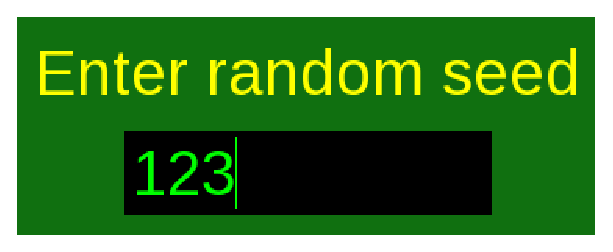
\epsfig{file=seedentry.eps,width=1.45in}
\end{minipage}

The return value from {\tt set\_seed} indicates whether the input string
did in fact correspond to a number.  When the string represents
a number, the function returns~1.
Otherwise, the function returns~0.

We use fixed seeds in
this assignment because a fixed seed produces a fixed sequence of 
random numbers, which means that the solution code will always be the
same.  Determinism makes debugging much easier---imagine trying to find
a bug that only appears in one run out of every million.  Once you have
debugged your code (but {\bf not in the version that you submit for grading}),
feel free to change the random seed to be, for example, time-based
({\tt srand (time (NULL));}), 
so as to provide a more realistic feeling of randomness.

\pagebreak

Now let's consider the part that you must do alone.
%
Here are function signatures for the two functions:\vspace{-8pt}

{\tt
\begin{tabbing}
~~~~\=int32\_t start\_game (int32\_t* one, int32\_t* two, int32\_t* three, int32\_t* four);\\
\>int32\_t make\_guess (\=const char* guess\_str, int32\_t* one, int32\_t* two, int32\_t* three,\\
\>\>int32\_t* four);
\end{tabbing}
}\vspace{-8pt}

The {\tt start\_game} routine selects the solution code, a set of four
numbers from~1 to~8.  To ensure consistency between your program's output
and ours, you {\bf must use the algorithm on the next page} for generating the
solution code.\vspace{-8pt}

\begin{list}{x}{\setlength{\leftmargin}{1.25in}\setlength{\rightmargin}{0.5in}\setlength{\labelwidth}{1in}\setlength{\itemsep}{0pt}\setlength{\parskip}{0pt}\setlength{\parsep}{0pt}}
\item[{\bf Step 1:}]{Starting with the first value in the code
sequence, generate a random integer in the range~0 to~7 inclusive
using a single call to {\tt rand} and a single modulus~({\tt \%}) operator.}
\item[{\bf Step 2:}]{Add 1 to the resulting number to get a value in the
range~1 to~8.}
\item[{\bf Step 3:}]{Repeat for the other three solution code 
values (in order).}
\end{list}\vspace{-8pt}

You must also make your own copy of the solution code using file-scoped
variables.  This copy will be necessary when you implement {\tt make\_guess}.

Be sure not to call {\tt srand} outside of the {\tt set\_seed} function
and not to call {\tt rand} outside of the {\tt start\_game} function.
Calling either of these disrupts the sequence of random numbers and will
cause your output to differ from ours.  Please also be aware that {\bf the
pseudo-random number generators on Linux and Android are different}, 
so the same 
random seed will produce different solution codes on the lab machine and 
your Android device.

Finally, you must write the {\tt make\_guess} routine that compares a
player's guess with the solution.  The inputs to this routine include
a string (the player's input) 
and four pointers to integers. 
%
Your routine must validate the string in the same way that we did for 
{\tt set\_seed}.  A valid string contains exactly four numbers (and no
extra garbage at the end).
All four numbers in the string must be between~1 and~8.
If the string is invalid, your routine must print an error
message, ``{\tt set\_seed:~invalid~seed$\backslash$n}'', then return 0.  

For a valid string, you must store a copy of the guessed code {\em in order}
in the four addresses provided as input parameters.
%
Your routine must then compare the guessed code with the solution code
to count the number of perfect and misplaced matches, then print a message
informing the player of the results.

Let's consider some examples.  Imagine that the solution code is {\tt 1~1~2~3}.
If the player guesses {\tt 1~2~2~4}, the first~(leftmost) and third code
values match perfectly, so they have two perfect matches.  How many
misplaced matches does this guess have?  Think of the solution and guess
code values as being paired with one another.  If we pair two values as 
a perfect match, neither of these values can be paired with another value.
So the {\tt 1} in the guess does not produce a misplaced match: the
{\tt 1} in the guess has
already been paired with the first {\tt 1} in the solution.  Neither does
the first~(left) {\tt 2} in the guess produce a misplaced match: the
{\tt 2} in the solution has already been paired with the other {\tt 2} 
in the guess.  Perfect matches are always paired before misplaced matches,
so there is never any ambiguity.  If you are in doubt, use the test code
that we have provided to check your answers on the lab machines.

What happens if (using the same solution code: {\tt 1~1~2~3}) the user
guesses~{\tt 4~4~1~1}?  Here they have no perfect matches.  How many
misplaced matches does the guess code have?  Keep the pairing idea in
mind.  We can pair either of the {\tt 1}'s in the guess with the {\tt 1}'s
in the solution, but we have exactly two pairs, and thus we must report
exactly two misplaced matches.

Once your routine has calculated the number of perfect and misplaced
matches, it must print a message using exactly the format shown here
(without the quotes):

\protect{\mbox{\hspace{.25in}}}%
``{\tt With guess 1, you got 1 perfect matches and 2 misplaced matches.$\backslash$n}''

The guess number starts at~1 and goes up as high as 12---your code
must also track this value using a file-scoped variable.  Note that
only valid guesses count as turns.  Do not adjust the word ``matches''
for subject-verb agreement.

The {\tt make\_guess} routine should return~1 when the user has provided
a valid guess string.\\


\pagebreak

\classsect{Challenges for Program 5}

Here are some challenges for this week.  You can find the function
signatures in the header or the source file.  You can test correct
behavior in the Android demo package (see the web page).  For the
challenges, you must
either write your own tests or use the graphical version to test
on the lab machines.

\begin{list}{x}{\setlength{\leftmargin}{1.25in}\setlength{\rightmargin}{0.5in}\setlength{\labelwidth}{.75in}\setlength{\itemsep}{0pt}\setlength{\parskip}{0pt}\setlength{\parsep}{0pt}}
\item[{\bf (8~points)}]{Implement {\tt compare\_guesses}, which
checks whether a guess that the user is considering could be the
solution, based on a previous guess and the feedback (number of
perfect and misplaced matches) given for the previous guess.
For this function, all information is provided to you.  If you
implement it correctly, this challenge should be pretty easy,
so make sure that you think about your strategy.  Be aware that
the guess being considered may not be complete: values can be~0
rather than in the range~1 to~8.}
\item[{\bf (12~points)}]{(REQUIRES PREVIOUS CHALLENGE)
Implement {\tt get\_hint}, which
provides a sample code (four values) that is consistent
with all previous guesses (in other words, {\tt compare\_guesses}
returns~1 for all previous guesses made during this game).
You will need to add code to track those guesses yourself.
Note that one easy and accurate hint is to simply provide the
solution: {\bf NO CREDIT WILL BE GIVEN} for that approach.}
\end{list}\vspace{-12pt}


\classsect{Specifics}\vspace{4pt}

\begin{list}{$\bullet$}{\setlength{\itemsep}{0pt}\setlength{\parskip}{0pt}%
\setlength{\topsep}{0pt}\setlength{\partopsep}{0pt}\setlength{\parsep}{0pt}}
\item{Your code must be written in~C and
and must be contained in the {\tt prog5.c} file provided to you --- 
we will NOT grade files with any other name.}
\item{You must implement {\tt set\_seed}, {\tt start\_game}, and 
{\tt make\_guess} correctly.}
\item{Your routine's return values and outputs must match the gold version's 
exactly for full credit.}
\item{Your code must be well-commented.  You may use either \mbox{C-style}
({\tt /* can span multiple lines */}) or \mbox{C++-style}
({\tt // comment to end of line}) comments, as you prefer.
Follow the commenting style of 
the code examples provided in class and in the textbook. }
\end{list}\vspace{12pt}


\classsect{Building and Testing}

We suggest that you begin by developing your code using the text version
of the game on the Linux machines
in the lab.
As with Program~4, all operations mentioned here should be performed from 
your {\tt prog5}
directory, not from the {\tt jni} subdirectory that contains the file
with your code.

You should test your program thoroughly before handing in your solution.
We have provided you a set of tests with the text version, but nothing
specifically for the challenges.
You should get in the habit of writing your own tests.
%
To compile the {\tt text\_version.c} file, type

\protect{\mbox{\hspace{.25in}}}%
{\tt gcc -g -Wall text\_version.c}

If successful, the compiler produces an executable called {\tt a.out},
which you can execute by typing ``{\tt ./a.out}'' (no quotes).
%
You can also run the code with the {\tt gdb} debugger (or a GUI interface
that uses it, such as DDD) by typing:

\protect{\mbox{\hspace{.25in}}}%
{\tt gdb a.out}

The {\tt text-examples} subdirectory contains a gold version of the
text-based variant along with some sample input and output files.
These are not scripts, but direct input.  If you want to produce another
copy of {\tt output1}, you can execute the gold version (from within
the {\tt text-examples} directory) by typing:

\protect{\mbox{\hspace{.25in}}}%
{\tt ./text-version-gold < input1 > output1-copy}

The {\tt output1-copy} file then matches the {\tt output1} file provided 
exactly.  You can, of course, run your own program in the same way and
then use {\tt diff} to compare outputs.  You can also run the gold 
program on different inputs, if you are concerned about a particular test
case.  If you set your random seed correctly, you should not have 
difficulty getting the gold version to produce a solution code that you
know in advance.  You can also run it with twelve identical
guesses, since the game prints out the solution if the player loses.\\


\pagebreak

\classsect{Grading Rubric}
%
\begin{tabbing}
\textit{Func}\=\textit{tionality} (65\%)\\
  \>10\% - {\tt set\_seed} function works correctly\\
  \>10\% - {\tt start\_game} function works correctly\\
  \>40\% - {\tt make\_guess} function works correctly\\
  \>5\% - all outputs match exactly\\
\textit{Style (15\%)}\\
  \>5\% - compilation generates no warnings (note: any warning means 0 points here)\\
  \>5\% - does not use global variables (file-scoped are necessary)\\
  \>5\% -~\=indentation and variable names are appropriate and reasonably meaningful\\
  \>\>(index variables can be single-letter)\\
\textit{Comments, clarity, and write-up (20\%)}\\
  \> 5\% - introductory paragraph explaining what you did (even if it's just the required work)\\
  \>15\% - code is clear and well-commented
\end{tabbing}\vspace{-8pt}

Note that some point categories in the rubric may depend on other categories.
If your code does not compile, you may receive a score close to~0~points.

\end{document}
